\section{Simulation}
	
	\subsection{Anforderungen I}
	\begin{frame}{Simulation}{Anforderungen}
	  \begin{itemize}
	    \item Kommunikation mit GUI
	    \item Simulation in Echtzeit
	    \item Kommunikation mittels serieller Schnittstelle
	  \end{itemize}
	\end{frame}

	\subsection{Entwurf I}
	\begin{frame}{Simulation}{Entwurfsphase und Implementierung I}
	  	\begin{figure}[htbp]
	  		\centering
	  		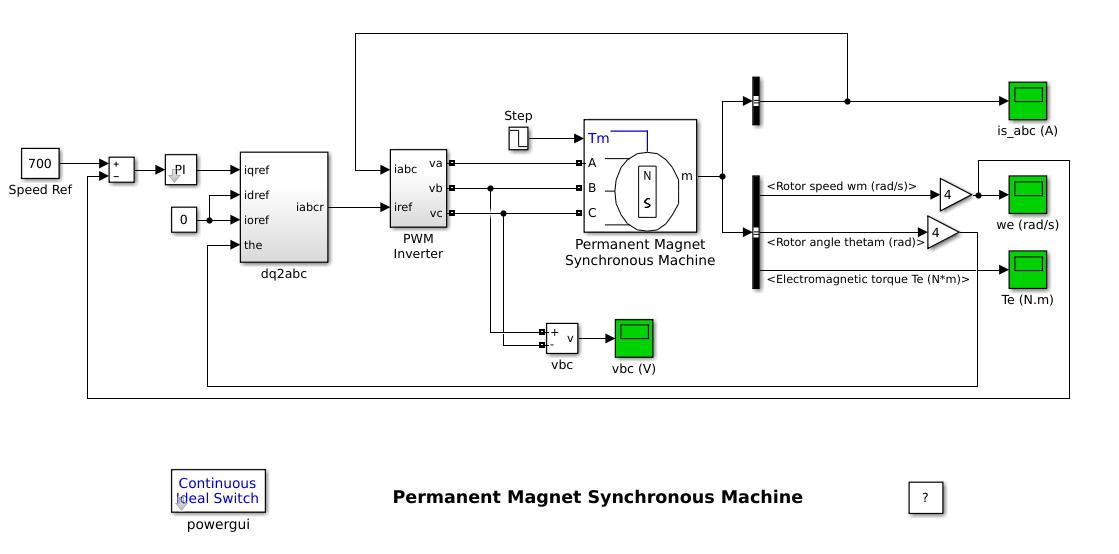
\includegraphics[width=\textwidth]{../sim/pictures/powerPmmotor.png}
	  	\end{figure}
	\end{frame}

	\subsection{Analysephase II}
	\begin{frame}{Simulation}{Analysephase II}
		\begin{center}
		\begin{tabular}{cc}
			\begin{minipage}{0.4\textwidth} 
				\includestandalone[width=\textwidth]{../sim/pictures/motorAufbau}
			\end{minipage}	
			&  
			\begin{minipage}{0.4\textwidth}
				\vspace{-0.35cm}
				\includestandalone[width=0.9\textwidth]{../sim/pictures/vereinfachtesModell}	
			\end{minipage}	
			\\ 
		\end{tabular} 
	
		\vspace{0.5cm}
		\includestandalone[width=0.8\textwidth]{../sim/pictures/abgerolltesModell}
	\end{center}
	\end{frame}

	\subsection{Bewertung des neuen Modells}
	\begin{frame}{Simulation}{Bewertung}
		\begin{itemize}
			\item Resultierendes Spulenfeld
				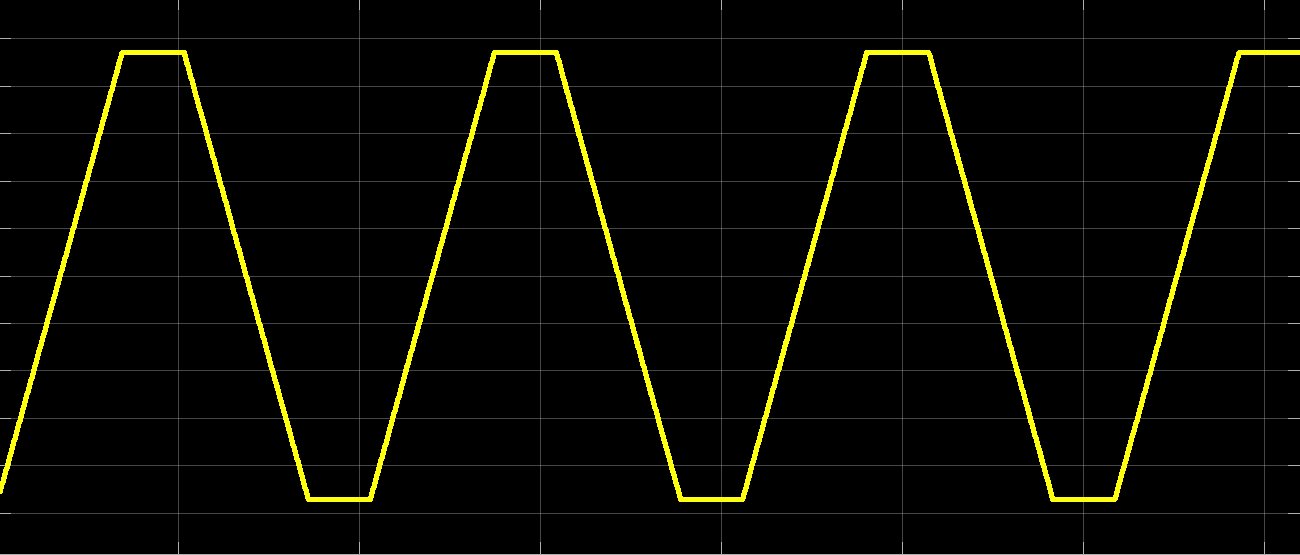
\includegraphics[width=0.8\textwidth]{../sim/pictures/resultierendesFeld.png}
				\newline
				$\sum \limits_1^{28} V_{res_i} = \sum \limits_1^{28} (V_i+R_i) = \sum \limits_1^{28} V_i + \sum \limits_1^{28} R_i$
		\end{itemize}	 
	\end{frame}

	\begin{frame}{Simulation}{Bewertung}
		\begin{itemize}
			\item Drehmoment
			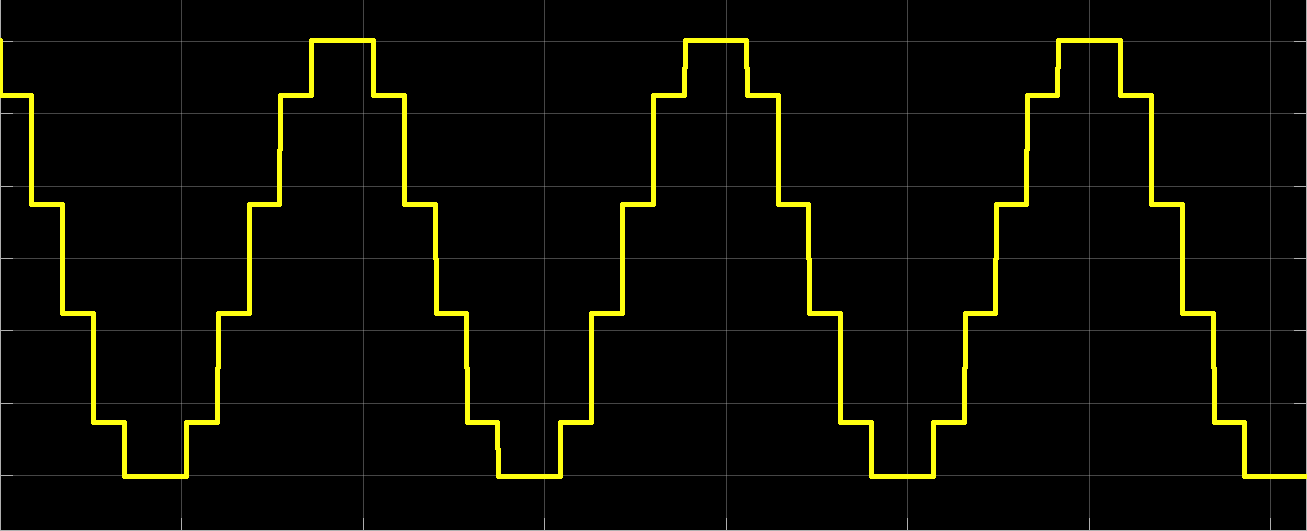
\includegraphics[width=0.8\textwidth]{../sim/pictures/drehmoment.png}
		\end{itemize}
	
	\end{frame}